\documentclass[twocolumn,10pt]{article}
\usepackage{amssymb}
\usepackage{amsmath}
\usepackage{amsfonts}
\usepackage{array,url,kantlipsum}
\usepackage{lineno,hyperref}
\usepackage{graphicx}
\usepackage{float}
\graphicspath{{../Figures/}}
\usepackage[margin=0.75in,tmargin=1in,bmargin=1in]{geometry}
\usepackage{array,multirow}
\usepackage{multirow}
\usepackage{tabu}
\usepackage[table]{xcolor}

\begin{document}
\twocolumn[{%
 \centering
 \LARGE New York City Taxi Data Exploration and Ride Prediction \\[0.5em]
 \large Kurt Nelson \\[1em]
 \normalsize
}]

\begin{abstract}
In this work we present the implementation of computer vision and machine learning to teach phones how to measure the volume of a poured liquid from video recordings. The ultimate goal is to develop a mobile application that removes the need for measuring cups in the kitchen by autonomously 1) storing ingredient measurements while food preparation is underway, or 2) instructing users on when to stop adding a particular ingredient. Experiments for data collection and feature extraction are outlined. We then present a model development and selection process that is applied to numerous regression and classification models for both volume prediction as a continuous random variable, and as a classification problem with labels increment in 1/4 cups. Of the regression models tested, locally weighted least squares regression performed best, with a test-data root mean squared error of 0.13 cup. For the classification models, Softmax regression performed best with a missclassification error of 25\%. Both models reduced prediction errors by a factor of 3 relative to approximate physics estimates.        
\end{abstract}

\section{Introduction}
Would you rather chew off your pinky finger or measure ingredients for the rest of your life? The response is unanimous; pinky's are overrated anyhow. No one likes measuring ingredients, but the Italian Grandma Method (IGM), adding a splash of this and a dab of that, produces gastronomical disasters for all but the most experienced chefs (e.g. IG’s). Many of us casual cooks are unable to reproduce winning recipes when applying the IGM, and instead are left with a one-hit-wonder followed by an onslaught of failed recreation attempts that litter our refrigerators with dreadful leftovers.


\section{Physics-based prediction}
Although machine learning has not been applied to measurement predictions in the kitchen, the volume of a poured liquid $V$ can be exactly computed from basic fluid dynamics if the velocity $v(x,y,t)$, cross-sectional area $A(x,y,t)$, and pour duration are known, viz. 
\begin{equation} \label{eq:1}
V = \iiint v(x,y,t) A(x,y,t) dx dz dt \\.
\end{equation}

\begin{figure}
\centering
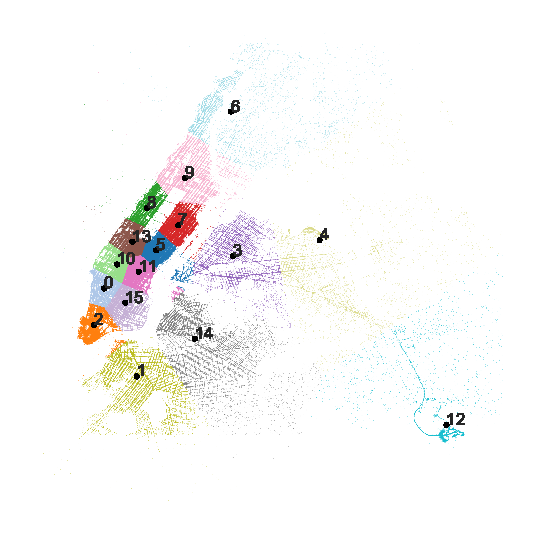
\includegraphics[width=90mm]{kMeansClusters}
\caption{K-means clustering.}
\label{fig:Clusters}
\end{figure}

\end{document}